\documentclass[1p]{elsarticle_modified}
%\bibliographystyle{elsarticle-num}

%\usepackage[colorlinks]{hyperref}
%\usepackage{abbrmath_seonhwa} %\Abb, \Ascr, \Acal ,\Abf, \Afrak
\usepackage{amsfonts}
\usepackage{amssymb}
\usepackage{amsmath}
\usepackage{amsthm}
\usepackage{scalefnt}
\usepackage{amsbsy}
\usepackage{kotex}
\usepackage{caption}
\usepackage{subfig}
\usepackage{color}
\usepackage{graphicx}
\usepackage{xcolor} %% white, black, red, green, blue, cyan, magenta, yellow
\usepackage{float}
\usepackage{setspace}
\usepackage{hyperref}

\usepackage{tikz}
\usetikzlibrary{arrows}

\usepackage{multirow}
\usepackage{array} % fixed length table
\usepackage{hhline}

%%%%%%%%%%%%%%%%%%%%%
\makeatletter
\renewcommand*\env@matrix[1][\arraystretch]{%
	\edef\arraystretch{#1}%
	\hskip -\arraycolsep
	\let\@ifnextchar\new@ifnextchar
	\array{*\c@MaxMatrixCols c}}
\makeatother %https://tex.stackexchange.com/questions/14071/how-can-i-increase-the-line-spacing-in-a-matrix
%%%%%%%%%%%%%%%

\usepackage[normalem]{ulem}

\newcommand{\msout}[1]{\ifmmode\text{\sout{\ensuremath{#1}}}\else\sout{#1}\fi}
%SOURCE: \msout is \stkout macro in https://tex.stackexchange.com/questions/20609/strikeout-in-math-mode

\newcommand{\cancel}[1]{
	\ifmmode
	{\color{red}\msout{#1}}
	\else
	{\color{red}\sout{#1}}
	\fi
}

\newcommand{\add}[1]{
	{\color{blue}\uwave{#1}}
}

\newcommand{\replace}[2]{
	\ifmmode
	{\color{red}\msout{#1}}{\color{blue}\uwave{#2}}
	\else
	{\color{red}\sout{#1}}{\color{blue}\uwave{#2}}
	\fi
}

\newcommand{\Sol}{\mathcal{S}} %segment
\newcommand{\D}{D} %diagram
\newcommand{\A}{\mathcal{A}} %arc


%%%%%%%%%%%%%%%%%%%%%%%%%%%%%5 test

\def\sl{\operatorname{\textup{SL}}(2,\Cbb)}
\def\psl{\operatorname{\textup{PSL}}(2,\Cbb)}
\def\quan{\mkern 1mu \triangleright \mkern 1mu}

\theoremstyle{definition}
\newtheorem{thm}{Theorem}[section]
\newtheorem{prop}[thm]{Proposition}
\newtheorem{lem}[thm]{Lemma}
\newtheorem{ques}[thm]{Question}
\newtheorem{cor}[thm]{Corollary}
\newtheorem{defn}[thm]{Definition}
\newtheorem{exam}[thm]{Example}
\newtheorem{rmk}[thm]{Remark}
\newtheorem{alg}[thm]{Algorithm}

\newcommand{\I}{\sqrt{-1}}
\begin{document}

%\begin{frontmatter}
%
%\title{Boundary parabolic representations of knots up to 8 crossings}
%
%%% Group authors per affiliation:
%\author{Yunhi Cho} 
%\address{Department of Mathematics, University of Seoul, Seoul, Korea}
%\ead{yhcho@uos.ac.kr}
%
%
%\author{Seonhwa Kim} %\fnref{s_kim}}
%\address{Center for Geometry and Physics, Institute for Basic Science, Pohang, 37673, Korea}
%\ead{ryeona17@ibs.re.kr}
%
%\author{Hyuk Kim}
%\address{Department of Mathematical Sciences, Seoul National University, Seoul 08826, Korea}
%\ead{hyukkim@snu.ac.kr}
%
%\author{Seokbeom Yoon}
%\address{Department of Mathematical Sciences, Seoul National University, Seoul, 08826,  Korea}
%\ead{sbyoon15@snu.ac.kr}
%
%\begin{abstract}
%We find all boundary parabolic representation of knots up to 8 crossings.
%
%\end{abstract}
%\begin{keyword}
%    \MSC[2010] 57M25 
%\end{keyword}
%
%\end{frontmatter}

%\linenumbers
%\tableofcontents
%
\newcommand\colored[1]{\textcolor{white}{\rule[-0.35ex]{0.8em}{1.4ex}}\kern-0.8em\color{red} #1}%
%\newcommand\colored[1]{\textcolor{white}{ #1}\kern-2.17ex	\textcolor{white}{ #1}\kern-1.81ex	\textcolor{white}{ #1}\kern-2.15ex\color{red}#1	}

{\Large $\underline{12a_{0177}~(K12a_{0177})}$}

\setlength{\tabcolsep}{10pt}
\renewcommand{\arraystretch}{1.6}
\vspace{1cm}\begin{tabular}{m{100pt}>{\centering\arraybackslash}m{274pt}}
\multirow{5}{120pt}{
	\centering
	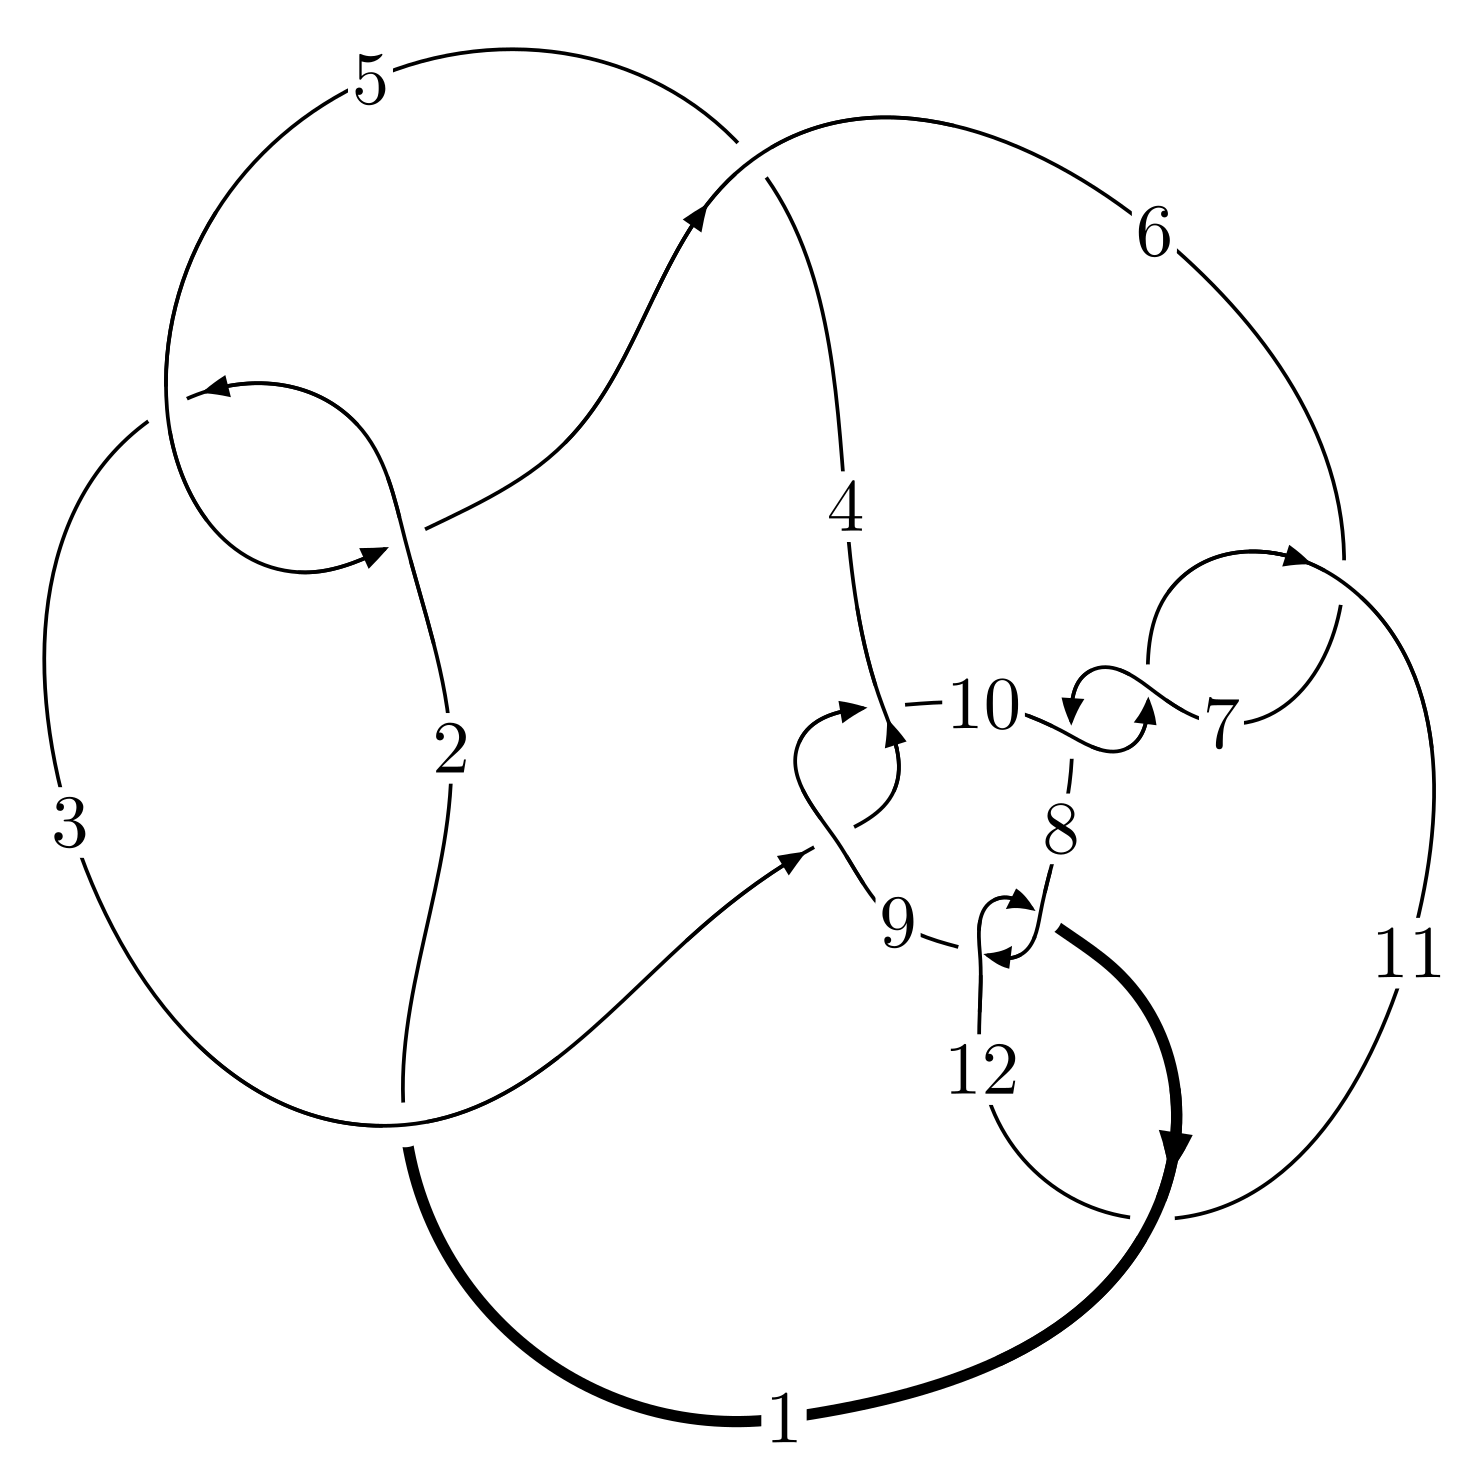
\includegraphics[width=112pt]{../../../GIT/diagram.site/Diagrams/png/978_12a_0177.png}\\
\ \ \ A knot diagram\footnotemark}&
\allowdisplaybreaks
\textbf{Linearized knot diagam} \\
\cline{2-2}
 &
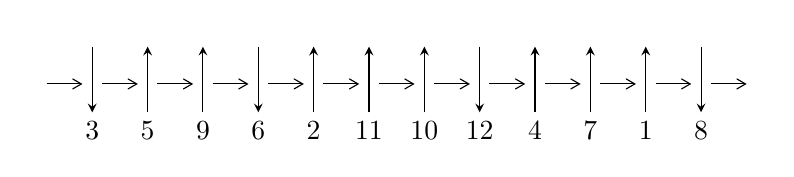
\begin{tikzpicture}[x=20pt, y=17pt]
	% nodes
	\node (C0) at (0, 0) {};
	\node (C1) at (1, 0) {};
	\node (C1U) at (1, +1) {};
	\node (C1D) at (1, -1) {3};

	\node (C2) at (2, 0) {};
	\node (C2U) at (2, +1) {};
	\node (C2D) at (2, -1) {5};

	\node (C3) at (3, 0) {};
	\node (C3U) at (3, +1) {};
	\node (C3D) at (3, -1) {9};

	\node (C4) at (4, 0) {};
	\node (C4U) at (4, +1) {};
	\node (C4D) at (4, -1) {6};

	\node (C5) at (5, 0) {};
	\node (C5U) at (5, +1) {};
	\node (C5D) at (5, -1) {2};

	\node (C6) at (6, 0) {};
	\node (C6U) at (6, +1) {};
	\node (C6D) at (6, -1) {11};

	\node (C7) at (7, 0) {};
	\node (C7U) at (7, +1) {};
	\node (C7D) at (7, -1) {10};

	\node (C8) at (8, 0) {};
	\node (C8U) at (8, +1) {};
	\node (C8D) at (8, -1) {12};

	\node (C9) at (9, 0) {};
	\node (C9U) at (9, +1) {};
	\node (C9D) at (9, -1) {4};

	\node (C10) at (10, 0) {};
	\node (C10U) at (10, +1) {};
	\node (C10D) at (10, -1) {7};

	\node (C11) at (11, 0) {};
	\node (C11U) at (11, +1) {};
	\node (C11D) at (11, -1) {1};

	\node (C12) at (12, 0) {};
	\node (C12U) at (12, +1) {};
	\node (C12D) at (12, -1) {8};
	\node (C13) at (13, 0) {};

	% arrows
	\draw[->,>={angle 60}]
	(C0) edge (C1) (C1) edge (C2) (C2) edge (C3) (C3) edge (C4) (C4) edge (C5) (C5) edge (C6) (C6) edge (C7) (C7) edge (C8) (C8) edge (C9) (C9) edge (C10) (C10) edge (C11) (C11) edge (C12) (C12) edge (C13) ;	\draw[->,>=stealth]
	(C1U) edge (C1D) (C2D) edge (C2U) (C3D) edge (C3U) (C4U) edge (C4D) (C5D) edge (C5U) (C6D) edge (C6U) (C7D) edge (C7U) (C8U) edge (C8D) (C9D) edge (C9U) (C10D) edge (C10U) (C11D) edge (C11U) (C12U) edge (C12D) ;
	\end{tikzpicture} \\
\hhline{~~} \\& 
\textbf{Solving Sequence} \\ \cline{2-2} 
 &
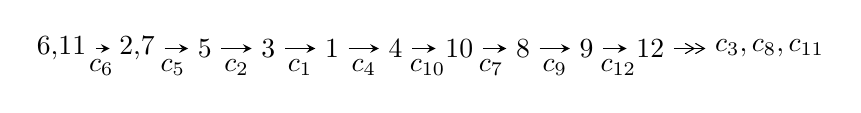
\begin{tikzpicture}[x=23pt, y=7pt]
	% node
	\node (A0) at (-1/8, 0) {6,11};
	\node (A1) at (17/16, 0) {2,7};
	\node (A2) at (17/8, 0) {5};
	\node (A3) at (25/8, 0) {3};
	\node (A4) at (33/8, 0) {1};
	\node (A5) at (41/8, 0) {4};
	\node (A6) at (49/8, 0) {10};
	\node (A7) at (57/8, 0) {8};
	\node (A8) at (65/8, 0) {9};
	\node (A9) at (73/8, 0) {12};
	\node (C1) at (1/2, -1) {$c_{6}$};
	\node (C2) at (13/8, -1) {$c_{5}$};
	\node (C3) at (21/8, -1) {$c_{2}$};
	\node (C4) at (29/8, -1) {$c_{1}$};
	\node (C5) at (37/8, -1) {$c_{4}$};
	\node (C6) at (45/8, -1) {$c_{10}$};
	\node (C7) at (53/8, -1) {$c_{7}$};
	\node (C8) at (61/8, -1) {$c_{9}$};
	\node (C9) at (69/8, -1) {$c_{12}$};
	\node (A10) at (11, 0) {$c_{3},c_{8},c_{11}$};

	% edge
	\draw[->,>=stealth]	
	(A0) edge (A1) (A1) edge (A2) (A2) edge (A3) (A3) edge (A4) (A4) edge (A5) (A5) edge (A6) (A6) edge (A7) (A7) edge (A8) (A8) edge (A9) ;
	\draw[->>,>={angle 60}]	
	(A9) edge (A10);
\end{tikzpicture} \\ 

\end{tabular} \\

\footnotetext{
The image of knot diagram is generated by the software ``\textbf{Draw programme}" developed by Andrew Bartholomew(\url{http://www.layer8.co.uk/maths/draw/index.htm\#Running-draw}), where we modified some parts for our purpose(\url{https://github.com/CATsTAILs/LinksPainter}).
}\phantom \\ \newline 
\centering \textbf{Ideals for irreducible components\footnotemark of $X_{\text{par}}$} 
 
\begin{align*}
I^u_{1}&=\langle 
7.32498\times10^{64} u^{73}+8.66991\times10^{64} u^{72}+\cdots+6.16277\times10^{65} b-4.73818\times10^{66},\\
\phantom{I^u_{1}}&\phantom{= \langle  }-1.00235\times10^{67} u^{73}-1.65925\times10^{67} u^{72}+\cdots+2.09534\times10^{67} a+3.92221\times10^{68},\\
\phantom{I^u_{1}}&\phantom{= \langle  }u^{74}+3 u^{73}+\cdots+241 u+34\rangle \\
I^u_{2}&=\langle 
- u^{12}-4 u^{10}+2 u^9-6 u^8+6 u^7-6 u^6+6 u^5-5 u^4+2 u^3-2 u^2+b,\\
\phantom{I^u_{2}}&\phantom{= \langle  }u^{10}+3 u^8-2 u^7+4 u^6-4 u^5+5 u^4-4 u^3+3 u^2+a-2 u+1,\;u^{27}+9 u^{25}+\cdots+u-1\rangle \\
I^u_{3}&=\langle 
u^2 a+u^2+b+a+1,\;2 u^3 a+4 u^2 a+5 u^3+4 a^2+6 a u+6 u^2+14 a+13 u+15,\;u^4+u^3+3 u^2+2 u+1\rangle \\
I^u_{4}&=\langle 
- a^2-2 a u+b+2 a+2 u-1,\;a^4+3 a^3 u-4 a^3-9 a^2 u+5 a^2+11 a u-2 a-5 u+1,\;u^2+1\rangle \\
\\
\end{align*}
\raggedright * 4 irreducible components of $\dim_{\mathbb{C}}=0$, with total 117 representations.\\
\footnotetext{All coefficients of polynomials are rational numbers. But the coefficients are sometimes approximated in decimal forms when there is not enough margin.}
\newpage
\renewcommand{\arraystretch}{1}
\centering \section*{I. $I^u_{1}= \langle 7.32\times10^{64} u^{73}+8.67\times10^{64} u^{72}+\cdots+6.16\times10^{65} b-4.74\times10^{66},\;-1.00\times10^{67} u^{73}-1.66\times10^{67} u^{72}+\cdots+2.10\times10^{67} a+3.92\times10^{68},\;u^{74}+3 u^{73}+\cdots+241 u+34 \rangle$}
\flushleft \textbf{(i) Arc colorings}\\
\begin{tabular}{m{7pt} m{180pt} m{7pt} m{180pt} }
\flushright $a_{6}=$&$\begin{pmatrix}1\\0\end{pmatrix}$ \\
\flushright $a_{11}=$&$\begin{pmatrix}0\\u\end{pmatrix}$ \\
\flushright $a_{2}=$&$\begin{pmatrix}0.478370 u^{73}+0.791874 u^{72}+\cdots-33.3429 u-18.7187\\-0.118859 u^{73}-0.140682 u^{72}+\cdots+21.7836 u+7.68839\end{pmatrix}$ \\
\flushright $a_{7}=$&$\begin{pmatrix}1\\- u^2\end{pmatrix}$ \\
\flushright $a_{5}=$&$\begin{pmatrix}-1.54482 u^{73}-3.80613 u^{72}+\cdots-519.075 u-88.4779\\0.760024 u^{73}+1.86639 u^{72}+\cdots+269.188 u+47.8263\end{pmatrix}$ \\
\flushright $a_{3}=$&$\begin{pmatrix}0.570211 u^{73}+1.31506 u^{72}+\cdots+144.190 u+26.0532\\0.0702357 u^{73}+0.201359 u^{72}+\cdots-19.1668 u-9.42275\end{pmatrix}$ \\
\flushright $a_{1}=$&$\begin{pmatrix}0.737803 u^{73}+1.93511 u^{72}+\cdots+256.366 u+47.4633\\0.565372 u^{73}+1.35960 u^{72}+\cdots+138.390 u+21.9622\end{pmatrix}$ \\
\flushright $a_{4}=$&$\begin{pmatrix}-0.784791 u^{73}-1.93974 u^{72}+\cdots-249.887 u-40.6516\\0.760024 u^{73}+1.86639 u^{72}+\cdots+269.188 u+47.8263\end{pmatrix}$ \\
\flushright $a_{10}=$&$\begin{pmatrix}- u\\u^3+u\end{pmatrix}$ \\
\flushright $a_{8}=$&$\begin{pmatrix}u^2+1\\- u^4-2 u^2\end{pmatrix}$ \\
\flushright $a_{9}=$&$\begin{pmatrix}1.26077 u^{73}+3.03039 u^{72}+\cdots+376.302 u+61.5916\\-1.04521 u^{73}-2.74727 u^{72}+\cdots-382.989 u-69.8736\end{pmatrix}$ \\
\flushright $a_{12}=$&$\begin{pmatrix}1.61959 u^{73}+4.23678 u^{72}+\cdots+593.454 u+111.477\\0.435515 u^{73}+0.883326 u^{72}+\cdots+44.5571 u+0.814681\end{pmatrix}$\\&\end{tabular}
\flushleft \textbf{(ii) Obstruction class $= -1$}\\~\\
\flushleft \textbf{(iii) Cusp Shapes $= 0.202194 u^{73}+0.134817 u^{72}+\cdots-112.657 u-17.5239$}\\~\\
\newpage\renewcommand{\arraystretch}{1}
\flushleft \textbf{(iv) u-Polynomials at the component}\newline \\
\begin{tabular}{m{50pt}|m{274pt}}
Crossings & \hspace{64pt}u-Polynomials at each crossing \\
\hline $$\begin{aligned}c_{1},c_{4}\end{aligned}$$&$\begin{aligned}
&u^{74}+24 u^{73}+\cdots-225 u+16
\end{aligned}$\\
\hline $$\begin{aligned}c_{2},c_{5}\end{aligned}$$&$\begin{aligned}
&u^{74}+4 u^{73}+\cdots+35 u+4
\end{aligned}$\\
\hline $$\begin{aligned}c_{3},c_{9}\end{aligned}$$&$\begin{aligned}
&u^{74}-2 u^{73}+\cdots-2560 u+2048
\end{aligned}$\\
\hline $$\begin{aligned}c_{6},c_{7},c_{10}\end{aligned}$$&$\begin{aligned}
&u^{74}+3 u^{73}+\cdots+241 u+34
\end{aligned}$\\
\hline $$\begin{aligned}c_{8},c_{12}\end{aligned}$$&$\begin{aligned}
&u^{74}+3 u^{73}+\cdots+243 u+34
\end{aligned}$\\
\hline $$\begin{aligned}c_{11}\end{aligned}$$&$\begin{aligned}
&u^{74}-31 u^{73}+\cdots-29555 u+1156
\end{aligned}$\\
\hline
\end{tabular}\\~\\
\newpage\renewcommand{\arraystretch}{1}
\flushleft \textbf{(v) Riley Polynomials at the component}\newline \\
\begin{tabular}{m{50pt}|m{274pt}}
Crossings & \hspace{64pt}Riley Polynomials at each crossing \\
\hline $$\begin{aligned}c_{1},c_{4}\end{aligned}$$&$\begin{aligned}
&y^{74}+56 y^{73}+\cdots+227743 y+256
\end{aligned}$\\
\hline $$\begin{aligned}c_{2},c_{5}\end{aligned}$$&$\begin{aligned}
&y^{74}+24 y^{73}+\cdots-225 y+16
\end{aligned}$\\
\hline $$\begin{aligned}c_{3},c_{9}\end{aligned}$$&$\begin{aligned}
&y^{74}-40 y^{73}+\cdots-36438016 y+4194304
\end{aligned}$\\
\hline $$\begin{aligned}c_{6},c_{7},c_{10}\end{aligned}$$&$\begin{aligned}
&y^{74}+75 y^{73}+\cdots+36099 y+1156
\end{aligned}$\\
\hline $$\begin{aligned}c_{8},c_{12}\end{aligned}$$&$\begin{aligned}
&y^{74}+31 y^{73}+\cdots+29555 y+1156
\end{aligned}$\\
\hline $$\begin{aligned}c_{11}\end{aligned}$$&$\begin{aligned}
&y^{74}+35 y^{73}+\cdots+11195711 y+1336336
\end{aligned}$\\
\hline
\end{tabular}\\~\\
\newpage\flushleft \textbf{(vi) Complex Volumes and Cusp Shapes}
$$\begin{array}{c|c|c}  
\text{Solutions to }I^u_{1}& \I (\text{vol} + \sqrt{-1}CS) & \text{Cusp shape}\\
 \hline 
\begin{aligned}
u &= -0.944775 + 0.259860 I \\
a &= \phantom{-}2.05390 - 0.30574 I \\
b &= -0.743584 + 1.028880 I\end{aligned}
 & \phantom{-}5.92126 - 12.56140 I & \phantom{-0.000000 } 0 \\ \hline\begin{aligned}
u &= -0.944775 - 0.259860 I \\
a &= \phantom{-}2.05390 + 0.30574 I \\
b &= -0.743584 - 1.028880 I\end{aligned}
 & \phantom{-}5.92126 + 12.56140 I & \phantom{-0.000000 } 0 \\ \hline\begin{aligned}
u &= -0.921296 + 0.218016 I \\
a &= \phantom{-}1.35216 + 1.03131 I \\
b &= -0.857448 - 0.692852 I\end{aligned}
 & \phantom{-}6.95372 - 6.59603 I & \phantom{-0.000000 } 0 \\ \hline\begin{aligned}
u &= -0.921296 - 0.218016 I \\
a &= \phantom{-}1.35216 - 1.03131 I \\
b &= -0.857448 + 0.692852 I\end{aligned}
 & \phantom{-}6.95372 + 6.59603 I & \phantom{-0.000000 } 0 \\ \hline\begin{aligned}
u &= \phantom{-}0.701992 + 0.812926 I \\
a &= \phantom{-}0.745443 - 0.467058 I \\
b &= -0.711125 + 0.915757 I\end{aligned}
 & \phantom{-}2.32200 - 1.76357 I & \phantom{-0.000000 } 0 \\ \hline\begin{aligned}
u &= \phantom{-}0.701992 - 0.812926 I \\
a &= \phantom{-}0.745443 + 0.467058 I \\
b &= -0.711125 - 0.915757 I\end{aligned}
 & \phantom{-}2.32200 + 1.76357 I & \phantom{-0.000000 } 0 \\ \hline\begin{aligned}
u &= \phantom{-}0.633453 + 0.888233 I \\
a &= \phantom{-}1.49188 - 0.19124 I \\
b &= -0.734625 - 0.820944 I\end{aligned}
 & \phantom{-}2.61817 + 3.75049 I & \phantom{-0.000000 } 0 \\ \hline\begin{aligned}
u &= \phantom{-}0.633453 - 0.888233 I \\
a &= \phantom{-}1.49188 + 0.19124 I \\
b &= -0.734625 + 0.820944 I\end{aligned}
 & \phantom{-}2.61817 - 3.75049 I & \phantom{-0.000000 } 0 \\ \hline\begin{aligned}
u &= -0.784151 + 0.296355 I \\
a &= -0.632018 + 0.069860 I \\
b &= \phantom{-}0.190621 - 1.095890 I\end{aligned}
 & -0.13573 - 6.54057 I & \phantom{-}4.00000 + 8.07439 I \\ \hline\begin{aligned}
u &= -0.784151 - 0.296355 I \\
a &= -0.632018 - 0.069860 I \\
b &= \phantom{-}0.190621 + 1.095890 I\end{aligned}
 & -0.13573 + 6.54057 I & \phantom{-}4.00000 - 8.07439 I\\
 \hline 
 \end{array}$$\newpage$$\begin{array}{c|c|c}  
\text{Solutions to }I^u_{1}& \I (\text{vol} + \sqrt{-1}CS) & \text{Cusp shape}\\
 \hline 
\begin{aligned}
u &= \phantom{-}0.672265 + 0.482118 I \\
a &= \phantom{-}1.222840 + 0.018497 I \\
b &= -0.042473 - 0.877998 I\end{aligned}
 & -1.54681 + 2.12225 I & \phantom{-0.000000 } 0. - 3.10049 I \\ \hline\begin{aligned}
u &= \phantom{-}0.672265 - 0.482118 I \\
a &= \phantom{-}1.222840 - 0.018497 I \\
b &= -0.042473 + 0.877998 I\end{aligned}
 & -1.54681 - 2.12225 I & \phantom{-0.000000 -}0. + 3.10049 I \\ \hline\begin{aligned}
u &= -0.126360 + 1.199890 I \\
a &= \phantom{-}1.040200 + 0.208918 I \\
b &= -0.877658 - 0.958922 I\end{aligned}
 & \phantom{-}6.07360 + 1.90106 I & \phantom{-0.000000 } 0 \\ \hline\begin{aligned}
u &= -0.126360 - 1.199890 I \\
a &= \phantom{-}1.040200 - 0.208918 I \\
b &= -0.877658 + 0.958922 I\end{aligned}
 & \phantom{-}6.07360 - 1.90106 I & \phantom{-0.000000 } 0 \\ \hline\begin{aligned}
u &= \phantom{-}0.114557 + 0.782746 I \\
a &= \phantom{-}0.659521 + 0.464671 I \\
b &= \phantom{-}0.177178 + 0.779440 I\end{aligned}
 & -1.59283 + 1.64325 I & -3.33878 - 4.86673 I \\ \hline\begin{aligned}
u &= \phantom{-}0.114557 - 0.782746 I \\
a &= \phantom{-}0.659521 - 0.464671 I \\
b &= \phantom{-}0.177178 - 0.779440 I\end{aligned}
 & -1.59283 - 1.64325 I & -3.33878 + 4.86673 I \\ \hline\begin{aligned}
u &= -0.164572 + 1.204940 I \\
a &= \phantom{-}1.227960 - 0.069637 I \\
b &= -0.910018 + 0.882320 I\end{aligned}
 & \phantom{-}6.31241 - 4.67571 I & \phantom{-0.000000 } 0 \\ \hline\begin{aligned}
u &= -0.164572 - 1.204940 I \\
a &= \phantom{-}1.227960 + 0.069637 I \\
b &= -0.910018 - 0.882320 I\end{aligned}
 & \phantom{-}6.31241 + 4.67571 I & \phantom{-0.000000 } 0 \\ \hline\begin{aligned}
u &= \phantom{-}0.742648 + 0.206519 I \\
a &= -2.53072 - 1.14776 I \\
b &= \phantom{-}0.716663 + 0.940041 I\end{aligned}
 & \phantom{-}2.97428 + 6.29652 I & \phantom{-}7.50844 - 6.68334 I \\ \hline\begin{aligned}
u &= \phantom{-}0.742648 - 0.206519 I \\
a &= -2.53072 + 1.14776 I \\
b &= \phantom{-}0.716663 - 0.940041 I\end{aligned}
 & \phantom{-}2.97428 - 6.29652 I & \phantom{-}7.50844 + 6.68334 I\\
 \hline 
 \end{array}$$\newpage$$\begin{array}{c|c|c}  
\text{Solutions to }I^u_{1}& \I (\text{vol} + \sqrt{-1}CS) & \text{Cusp shape}\\
 \hline 
\begin{aligned}
u &= -0.717121 + 0.158800 I \\
a &= -1.225590 + 0.380080 I \\
b &= \phantom{-}0.731356 - 0.145206 I\end{aligned}
 & \phantom{-}3.98068 - 3.64075 I & \phantom{-}11.59299 + 4.80389 I \\ \hline\begin{aligned}
u &= -0.717121 - 0.158800 I \\
a &= -1.225590 - 0.380080 I \\
b &= \phantom{-}0.731356 + 0.145206 I\end{aligned}
 & \phantom{-}3.98068 + 3.64075 I & \phantom{-}11.59299 - 4.80389 I \\ \hline\begin{aligned}
u &= \phantom{-}0.668164 + 0.154518 I \\
a &= -2.39850 + 1.57549 I \\
b &= \phantom{-}0.744333 - 0.790073 I\end{aligned}
 & \phantom{-}3.43591 + 0.73188 I & \phantom{-}9.08233 - 1.08851 I \\ \hline\begin{aligned}
u &= \phantom{-}0.668164 - 0.154518 I \\
a &= -2.39850 - 1.57549 I \\
b &= \phantom{-}0.744333 + 0.790073 I\end{aligned}
 & \phantom{-}3.43591 - 0.73188 I & \phantom{-}9.08233 + 1.08851 I \\ \hline\begin{aligned}
u &= -0.129344 + 1.322690 I \\
a &= -0.479899 - 0.769382 I \\
b &= \phantom{-}0.779061 + 0.657588 I\end{aligned}
 & -3.18435 + 0.63847 I & \phantom{-0.000000 } 0 \\ \hline\begin{aligned}
u &= -0.129344 - 1.322690 I \\
a &= -0.479899 + 0.769382 I \\
b &= \phantom{-}0.779061 - 0.657588 I\end{aligned}
 & -3.18435 - 0.63847 I & \phantom{-0.000000 } 0 \\ \hline\begin{aligned}
u &= \phantom{-}0.168573 + 1.321110 I \\
a &= -0.405207 + 0.035030 I \\
b &= \phantom{-}0.761529 + 0.328332 I\end{aligned}
 & -2.90837 + 2.42803 I & \phantom{-0.000000 } 0 \\ \hline\begin{aligned}
u &= \phantom{-}0.168573 - 1.321110 I \\
a &= -0.405207 - 0.035030 I \\
b &= \phantom{-}0.761529 - 0.328332 I\end{aligned}
 & -2.90837 - 2.42803 I & \phantom{-0.000000 } 0 \\ \hline\begin{aligned}
u &= -0.619119 + 0.176034 I \\
a &= \phantom{-}0.73745 + 1.54337 I \\
b &= -0.846329 - 0.820584 I\end{aligned}
 & \phantom{-}9.31962 + 1.94114 I & \phantom{-}12.61811 - 2.00223 I \\ \hline\begin{aligned}
u &= -0.619119 - 0.176034 I \\
a &= \phantom{-}0.73745 - 1.54337 I \\
b &= -0.846329 + 0.820584 I\end{aligned}
 & \phantom{-}9.31962 - 1.94114 I & \phantom{-}12.61811 + 2.00223 I\\
 \hline 
 \end{array}$$\newpage$$\begin{array}{c|c|c}  
\text{Solutions to }I^u_{1}& \I (\text{vol} + \sqrt{-1}CS) & \text{Cusp shape}\\
 \hline 
\begin{aligned}
u &= \phantom{-}0.080972 + 1.372850 I \\
a &= -0.741831 - 0.900405 I \\
b &= \phantom{-}0.543374 - 1.089860 I\end{aligned}
 & -5.16943 - 2.42403 I & \phantom{-0.000000 } 0 \\ \hline\begin{aligned}
u &= \phantom{-}0.080972 - 1.372850 I \\
a &= -0.741831 + 0.900405 I \\
b &= \phantom{-}0.543374 + 1.089860 I\end{aligned}
 & -5.16943 + 2.42403 I & \phantom{-0.000000 } 0 \\ \hline\begin{aligned}
u &= -0.195770 + 1.365850 I \\
a &= -1.82469 - 0.71360 I \\
b &= \phantom{-}0.693804 - 1.006320 I\end{aligned}
 & -4.22851 - 4.92303 I & \phantom{-0.000000 } 0 \\ \hline\begin{aligned}
u &= -0.195770 - 1.365850 I \\
a &= -1.82469 + 0.71360 I \\
b &= \phantom{-}0.693804 + 1.006320 I\end{aligned}
 & -4.22851 + 4.92303 I & \phantom{-0.000000 } 0 \\ \hline\begin{aligned}
u &= \phantom{-}0.264758 + 1.357650 I \\
a &= -0.734404 + 0.940199 I \\
b &= \phantom{-}0.834563 - 0.756749 I\end{aligned}
 & -1.35573 + 4.11982 I & \phantom{-0.000000 } 0 \\ \hline\begin{aligned}
u &= \phantom{-}0.264758 - 1.357650 I \\
a &= -0.734404 - 0.940199 I \\
b &= \phantom{-}0.834563 + 0.756749 I\end{aligned}
 & -1.35573 - 4.11982 I & \phantom{-0.000000 } 0 \\ \hline\begin{aligned}
u &= -0.287291 + 1.361710 I \\
a &= -0.635754 - 0.259327 I \\
b &= \phantom{-}0.855562 - 0.209147 I\end{aligned}
 & -0.83655 - 7.27459 I & \phantom{-0.000000 } 0 \\ \hline\begin{aligned}
u &= -0.287291 - 1.361710 I \\
a &= -0.635754 + 0.259327 I \\
b &= \phantom{-}0.855562 + 0.209147 I\end{aligned}
 & -0.83655 + 7.27459 I & \phantom{-0.000000 } 0 \\ \hline\begin{aligned}
u &= -0.221792 + 1.376420 I \\
a &= -0.337020 + 0.630518 I \\
b &= \phantom{-}0.469813 + 1.138480 I\end{aligned}
 & -3.81286 - 2.52146 I & \phantom{-0.000000 } 0 \\ \hline\begin{aligned}
u &= -0.221792 - 1.376420 I \\
a &= -0.337020 - 0.630518 I \\
b &= \phantom{-}0.469813 - 1.138480 I\end{aligned}
 & -3.81286 + 2.52146 I & \phantom{-0.000000 } 0\\
 \hline 
 \end{array}$$\newpage$$\begin{array}{c|c|c}  
\text{Solutions to }I^u_{1}& \I (\text{vol} + \sqrt{-1}CS) & \text{Cusp shape}\\
 \hline 
\begin{aligned}
u &= -0.545845 + 0.228098 I \\
a &= \phantom{-}2.57811 + 0.51294 I \\
b &= -0.800509 + 0.954675 I\end{aligned}
 & \phantom{-}8.90634 - 4.18645 I & \phantom{-}12.18887 + 3.45540 I \\ \hline\begin{aligned}
u &= -0.545845 - 0.228098 I \\
a &= \phantom{-}2.57811 - 0.51294 I \\
b &= -0.800509 - 0.954675 I\end{aligned}
 & \phantom{-}8.90634 + 4.18645 I & \phantom{-}12.18887 - 3.45540 I \\ \hline\begin{aligned}
u &= -0.545719 + 0.215154 I \\
a &= -1.73543 - 0.37199 I \\
b &= \phantom{-}0.421570 + 1.033690 I\end{aligned}
 & \phantom{-}1.244170 + 0.336310 I & \phantom{-}9.44086 + 1.14384 I \\ \hline\begin{aligned}
u &= -0.545719 - 0.215154 I \\
a &= -1.73543 + 0.37199 I \\
b &= \phantom{-}0.421570 - 1.033690 I\end{aligned}
 & \phantom{-}1.244170 - 0.336310 I & \phantom{-}9.44086 - 1.14384 I \\ \hline\begin{aligned}
u &= \phantom{-}0.29962 + 1.38522 I \\
a &= -1.98098 + 0.41163 I \\
b &= \phantom{-}0.755945 + 0.990941 I\end{aligned}
 & -2.08327 + 10.07100 I & \phantom{-0.000000 } 0 \\ \hline\begin{aligned}
u &= \phantom{-}0.29962 - 1.38522 I \\
a &= -1.98098 - 0.41163 I \\
b &= \phantom{-}0.755945 - 0.990941 I\end{aligned}
 & -2.08327 - 10.07100 I & \phantom{-0.000000 } 0 \\ \hline\begin{aligned}
u &= \phantom{-}0.07395 + 1.42707 I \\
a &= \phantom{-}0.701838 - 0.037664 I \\
b &= -0.569204 + 0.123347 I\end{aligned}
 & -5.46924 + 2.64105 I & \phantom{-0.000000 } 0 \\ \hline\begin{aligned}
u &= \phantom{-}0.07395 - 1.42707 I \\
a &= \phantom{-}0.701838 + 0.037664 I \\
b &= -0.569204 - 0.123347 I\end{aligned}
 & -5.46924 - 2.64105 I & \phantom{-0.000000 } 0 \\ \hline\begin{aligned}
u &= \phantom{-}0.21382 + 1.43929 I \\
a &= -0.487788 + 1.212470 I \\
b &= \phantom{-}0.120316 + 1.133060 I\end{aligned}
 & -7.79078 + 4.88573 I & \phantom{-0.000000 } 0 \\ \hline\begin{aligned}
u &= \phantom{-}0.21382 - 1.43929 I \\
a &= -0.487788 - 1.212470 I \\
b &= \phantom{-}0.120316 - 1.133060 I\end{aligned}
 & -7.79078 - 4.88573 I & \phantom{-0.000000 } 0\\
 \hline 
 \end{array}$$\newpage$$\begin{array}{c|c|c}  
\text{Solutions to }I^u_{1}& \I (\text{vol} + \sqrt{-1}CS) & \text{Cusp shape}\\
 \hline 
\begin{aligned}
u &= -0.31083 + 1.42891 I \\
a &= -0.828824 - 0.998794 I \\
b &= \phantom{-}0.177740 - 1.175180 I\end{aligned}
 & -5.64512 - 10.50590 I & \phantom{-0.000000 } 0 \\ \hline\begin{aligned}
u &= -0.31083 - 1.42891 I \\
a &= -0.828824 + 0.998794 I \\
b &= \phantom{-}0.177740 + 1.175180 I\end{aligned}
 & -5.64512 + 10.50590 I & \phantom{-0.000000 } 0 \\ \hline\begin{aligned}
u &= \phantom{-}0.33404 + 1.42646 I \\
a &= \phantom{-}0.275691 - 0.575217 I \\
b &= -0.839583 + 0.641379 I\end{aligned}
 & -1.11669 + 5.57868 I & \phantom{-0.000000 } 0 \\ \hline\begin{aligned}
u &= \phantom{-}0.33404 - 1.42646 I \\
a &= \phantom{-}0.275691 + 0.575217 I \\
b &= -0.839583 - 0.641379 I\end{aligned}
 & -1.11669 - 5.57868 I & \phantom{-0.000000 } 0 \\ \hline\begin{aligned}
u &= \phantom{-}0.343987 + 0.408307 I \\
a &= \phantom{-}1.259340 - 0.200200 I \\
b &= -0.164430 + 0.105291 I\end{aligned}
 & \phantom{-}0.438180 + 1.277440 I & \phantom{-}4.77216 - 5.31124 I \\ \hline\begin{aligned}
u &= \phantom{-}0.343987 - 0.408307 I \\
a &= \phantom{-}1.259340 + 0.200200 I \\
b &= -0.164430 - 0.105291 I\end{aligned}
 & \phantom{-}0.438180 - 1.277440 I & \phantom{-}4.77216 + 5.31124 I \\ \hline\begin{aligned}
u &= -0.38671 + 1.41560 I \\
a &= \phantom{-}0.358467 + 0.797877 I \\
b &= -0.900022 - 0.655211 I\end{aligned}
 & \phantom{-}1.77264 - 11.28690 I & \phantom{-0.000000 } 0 \\ \hline\begin{aligned}
u &= -0.38671 - 1.41560 I \\
a &= \phantom{-}0.358467 - 0.797877 I \\
b &= -0.900022 + 0.655211 I\end{aligned}
 & \phantom{-}1.77264 + 11.28690 I & \phantom{-0.000000 } 0 \\ \hline\begin{aligned}
u &= -0.39335 + 1.44216 I \\
a &= \phantom{-}1.78767 + 0.81460 I \\
b &= -0.744553 + 1.062820 I\end{aligned}
 & \phantom{-}0.5121 - 17.3690 I & \phantom{-0.000000 } 0 \\ \hline\begin{aligned}
u &= -0.39335 - 1.44216 I \\
a &= \phantom{-}1.78767 - 0.81460 I \\
b &= -0.744553 - 1.062820 I\end{aligned}
 & \phantom{-}0.5121 + 17.3690 I & \phantom{-0.000000 } 0\\
 \hline 
 \end{array}$$\newpage$$\begin{array}{c|c|c}  
\text{Solutions to }I^u_{1}& \I (\text{vol} + \sqrt{-1}CS) & \text{Cusp shape}\\
 \hline 
\begin{aligned}
u &= -0.07337 + 1.49652 I \\
a &= \phantom{-}0.689010 + 1.074630 I \\
b &= -0.098684 + 1.018160 I\end{aligned}
 & -9.15376 + 0.69582 I & \phantom{-0.000000 } 0 \\ \hline\begin{aligned}
u &= -0.07337 - 1.49652 I \\
a &= \phantom{-}0.689010 - 1.074630 I \\
b &= -0.098684 - 1.018160 I\end{aligned}
 & -9.15376 - 0.69582 I & \phantom{-0.000000 } 0 \\ \hline\begin{aligned}
u &= \phantom{-}0.33300 + 1.47174 I \\
a &= \phantom{-}1.55926 - 0.90181 I \\
b &= -0.717365 - 1.043070 I\end{aligned}
 & -2.33369 + 11.39850 I & \phantom{-0.000000 } 0 \\ \hline\begin{aligned}
u &= \phantom{-}0.33300 - 1.47174 I \\
a &= \phantom{-}1.55926 + 0.90181 I \\
b &= -0.717365 + 1.043070 I\end{aligned}
 & -2.33369 - 11.39850 I & \phantom{-0.000000 } 0 \\ \hline\begin{aligned}
u &= \phantom{-}0.20232 + 1.50188 I \\
a &= \phantom{-}1.013920 - 0.861496 I \\
b &= -0.197794 - 0.951591 I\end{aligned}
 & -8.06757 + 5.26507 I & \phantom{-0.000000 } 0 \\ \hline\begin{aligned}
u &= \phantom{-}0.20232 - 1.50188 I \\
a &= \phantom{-}1.013920 + 0.861496 I \\
b &= -0.197794 + 0.951591 I\end{aligned}
 & -8.06757 - 5.26507 I & \phantom{-0.000000 } 0 \\ \hline\begin{aligned}
u &= -0.152162 + 0.459797 I \\
a &= -3.15294 + 1.05533 I \\
b &= \phantom{-}0.535113 - 0.935355 I\end{aligned}
 & \phantom{-}0.28773 - 2.82692 I & \phantom{-}5.81058 - 1.66051 I \\ \hline\begin{aligned}
u &= -0.152162 - 0.459797 I \\
a &= -3.15294 - 1.05533 I \\
b &= \phantom{-}0.535113 + 0.935355 I\end{aligned}
 & \phantom{-}0.28773 + 2.82692 I & \phantom{-}5.81058 + 1.66051 I \\ \hline\begin{aligned}
u &= \phantom{-}0.04801 + 1.62342 I \\
a &= \phantom{-}0.686356 - 0.660507 I \\
b &= -0.622151 - 0.909091 I\end{aligned}
 & -6.42773 + 5.85172 I & \phantom{-0.000000 } 0 \\ \hline\begin{aligned}
u &= \phantom{-}0.04801 - 1.62342 I \\
a &= \phantom{-}0.686356 + 0.660507 I \\
b &= -0.622151 + 0.909091 I\end{aligned}
 & -6.42773 - 5.85172 I & \phantom{-0.000000 } 0\\
 \hline 
 \end{array}$$\newpage$$\begin{array}{c|c|c}  
\text{Solutions to }I^u_{1}& \I (\text{vol} + \sqrt{-1}CS) & \text{Cusp shape}\\
 \hline 
\begin{aligned}
u &= \phantom{-}0.11130 + 1.62165 I \\
a &= \phantom{-}0.478526 + 0.438391 I \\
b &= -0.614683 + 0.843469 I\end{aligned}
 & -6.20432 + 1.00932 I & \phantom{-0.000000 } 0 \\ \hline\begin{aligned}
u &= \phantom{-}0.11130 - 1.62165 I \\
a &= \phantom{-}0.478526 - 0.438391 I \\
b &= -0.614683 - 0.843469 I\end{aligned}
 & -6.20432 - 1.00932 I & \phantom{-0.000000 } 0 \\ \hline\begin{aligned}
u &= \phantom{-}0.012155 + 0.262876 I \\
a &= -2.05266 - 4.00172 I \\
b &= \phantom{-}0.483697 + 0.622554 I\end{aligned}
 & \phantom{-}1.18616 + 1.37603 I & \phantom{-}10.47248 - 4.16898 I \\ \hline\begin{aligned}
u &= \phantom{-}0.012155 - 0.262876 I \\
a &= -2.05266 + 4.00172 I \\
b &= \phantom{-}0.483697 - 0.622554 I\end{aligned}
 & \phantom{-}1.18616 - 1.37603 I & \phantom{-}10.47248 + 4.16898 I\\
 \hline 
 \end{array}$$\newpage\newpage\renewcommand{\arraystretch}{1}
\centering \section*{II. $I^u_{2}= \langle - u^{12}-4 u^{10}+\cdots-2 u^2+b,\;u^{10}+3 u^8+\cdots+a+1,\;u^{27}+9 u^{25}+\cdots+u-1 \rangle$}
\flushleft \textbf{(i) Arc colorings}\\
\begin{tabular}{m{7pt} m{180pt} m{7pt} m{180pt} }
\flushright $a_{6}=$&$\begin{pmatrix}1\\0\end{pmatrix}$ \\
\flushright $a_{11}=$&$\begin{pmatrix}0\\u\end{pmatrix}$ \\
\flushright $a_{2}=$&$\begin{pmatrix}- u^{10}-3 u^8+2 u^7-4 u^6+4 u^5-5 u^4+4 u^3-3 u^2+2 u-1\\u^{12}+4 u^{10}-2 u^9+6 u^8-6 u^7+6 u^6-6 u^5+5 u^4-2 u^3+2 u^2\end{pmatrix}$ \\
\flushright $a_{7}=$&$\begin{pmatrix}1\\- u^2\end{pmatrix}$ \\
\flushright $a_{5}=$&$\begin{pmatrix}- u^{22}-7 u^{20}+\cdots-2 u^2+1\\u^{24}+8 u^{22}+\cdots-8 u^5+4 u^4\end{pmatrix}$ \\
\flushright $a_{3}=$&$\begin{pmatrix}u^{21}+8 u^{19}+\cdots+6 u^3- u\\- u^{21}-7 u^{19}+\cdots- u^3+u\end{pmatrix}$ \\
\flushright $a_{1}=$&$\begin{pmatrix}- u\\u^3+u\end{pmatrix}$ \\
\flushright $a_{4}=$&$\begin{pmatrix}u^{24}+7 u^{22}+\cdots-2 u^2+1\\u^{24}+8 u^{22}+\cdots-8 u^5+4 u^4\end{pmatrix}$ \\
\flushright $a_{10}=$&$\begin{pmatrix}- u\\u^3+u\end{pmatrix}$ \\
\flushright $a_{8}=$&$\begin{pmatrix}u^2+1\\- u^4-2 u^2\end{pmatrix}$ \\
\flushright $a_{9}=$&$\begin{pmatrix}- u^4- u^2-1\\u^6+2 u^4+u^2\end{pmatrix}$ \\
\flushright $a_{12}=$&$\begin{pmatrix}u^3\\- u^5- u^3+u\end{pmatrix}$\\&\end{tabular}
\flushleft \textbf{(ii) Obstruction class $= -1$}\\~\\
\flushleft \textbf{(iii) Cusp Shapes $= 4 u^{24}+32 u^{22}-20 u^{21}+112 u^{20}-140 u^{19}+268 u^{18}-420 u^{17}+544 u^{16}-744 u^{15}+884 u^{14}-920 u^{13}+1000 u^{12}-860 u^{11}+724 u^{10}-556 u^9+316 u^8-168 u^7+60 u^6+28 u^5-24 u^4+24 u^3-16 u^2+10$}\\~\\
\newpage\renewcommand{\arraystretch}{1}
\flushleft \textbf{(iv) u-Polynomials at the component}\newline \\
\begin{tabular}{m{50pt}|m{274pt}}
Crossings & \hspace{64pt}u-Polynomials at each crossing \\
\hline $$\begin{aligned}c_{1},c_{4}\end{aligned}$$&$\begin{aligned}
&(u^9+3 u^8+8 u^7+13 u^6+17 u^5+17 u^4+12 u^3+6 u^2+u-1)^3
\end{aligned}$\\
\hline $$\begin{aligned}c_{2},c_{5}\end{aligned}$$&$\begin{aligned}
&(u^9+u^8+2 u^7+u^6+3 u^5+u^4+2 u^3+u-1)^3
\end{aligned}$\\
\hline $$\begin{aligned}c_{3},c_{9}\end{aligned}$$&$\begin{aligned}
&(u^9+u^8-2 u^7-3 u^6+u^5+3 u^4+2 u^3- u-1)^3
\end{aligned}$\\
\hline $$\begin{aligned}c_{6},c_{7},c_{8}\\c_{10},c_{12}\end{aligned}$$&$\begin{aligned}
&u^{27}+9 u^{25}+\cdots+u-1
\end{aligned}$\\
\hline $$\begin{aligned}c_{11}\end{aligned}$$&$\begin{aligned}
&u^{27}-18 u^{26}+\cdots+5 u+1
\end{aligned}$\\
\hline
\end{tabular}\\~\\
\newpage\renewcommand{\arraystretch}{1}
\flushleft \textbf{(v) Riley Polynomials at the component}\newline \\
\begin{tabular}{m{50pt}|m{274pt}}
Crossings & \hspace{64pt}Riley Polynomials at each crossing \\
\hline $$\begin{aligned}c_{1},c_{4}\end{aligned}$$&$\begin{aligned}
&(y^9+7 y^8+20 y^7+25 y^6+5 y^5-15 y^4+22 y^2+13 y-1)^3
\end{aligned}$\\
\hline $$\begin{aligned}c_{2},c_{5}\end{aligned}$$&$\begin{aligned}
&(y^9+3 y^8+8 y^7+13 y^6+17 y^5+17 y^4+12 y^3+6 y^2+y-1)^3
\end{aligned}$\\
\hline $$\begin{aligned}c_{3},c_{9}\end{aligned}$$&$\begin{aligned}
&(y^9-5 y^8+12 y^7-15 y^6+9 y^5+y^4-4 y^3+2 y^2+y-1)^3
\end{aligned}$\\
\hline $$\begin{aligned}c_{6},c_{7},c_{8}\\c_{10},c_{12}\end{aligned}$$&$\begin{aligned}
&y^{27}+18 y^{26}+\cdots+5 y-1
\end{aligned}$\\
\hline $$\begin{aligned}c_{11}\end{aligned}$$&$\begin{aligned}
&y^{27}-18 y^{26}+\cdots+25 y-1
\end{aligned}$\\
\hline
\end{tabular}\\~\\
\newpage\flushleft \textbf{(vi) Complex Volumes and Cusp Shapes}
$$\begin{array}{c|c|c}  
\text{Solutions to }I^u_{2}& \I (\text{vol} + \sqrt{-1}CS) & \text{Cusp shape}\\
 \hline 
\begin{aligned}
u &= \phantom{-}0.269474 + 1.004760 I \\
a &= -0.82716 + 1.96998 I \\
b &= \phantom{-}0.628449 - 0.875112 I\end{aligned}
 & \phantom{-}0.61694 - 2.45442 I & \phantom{-}2.32792 + 2.91298 I \\ \hline\begin{aligned}
u &= \phantom{-}0.269474 - 1.004760 I \\
a &= -0.82716 - 1.96998 I \\
b &= \phantom{-}0.628449 + 0.875112 I\end{aligned}
 & \phantom{-}0.61694 + 2.45442 I & \phantom{-}2.32792 - 2.91298 I \\ \hline\begin{aligned}
u &= \phantom{-}0.861055 + 0.381086 I \\
a &= \phantom{-}1.96932 + 0.07622 I \\
b &= -0.728966 - 0.986295 I\end{aligned}
 & \phantom{-}3.59813 + 7.08493 I & \phantom{-}5.57680 - 5.91335 I \\ \hline\begin{aligned}
u &= \phantom{-}0.861055 - 0.381086 I \\
a &= \phantom{-}1.96932 - 0.07622 I \\
b &= -0.728966 + 0.986295 I\end{aligned}
 & \phantom{-}3.59813 - 7.08493 I & \phantom{-}5.57680 + 5.91335 I \\ \hline\begin{aligned}
u &= -0.457598 + 0.805344 I \\
a &= \phantom{-}0.921794 + 0.293449 I \\
b &= \phantom{-}0.140343 + 0.966856 I\end{aligned}
 & -1.78344 + 2.09337 I & -0.51499 - 4.16283 I \\ \hline\begin{aligned}
u &= -0.457598 - 0.805344 I \\
a &= \phantom{-}0.921794 - 0.293449 I \\
b &= \phantom{-}0.140343 - 0.966856 I\end{aligned}
 & -1.78344 - 2.09337 I & -0.51499 + 4.16283 I \\ \hline\begin{aligned}
u &= \phantom{-}0.846765 + 0.300344 I \\
a &= \phantom{-}1.11197 - 0.96313 I \\
b &= -0.796005 + 0.733148 I\end{aligned}
 & \phantom{-}4.37135 + 1.33617 I & \phantom{-}7.28409 - 0.70175 I \\ \hline\begin{aligned}
u &= \phantom{-}0.846765 - 0.300344 I \\
a &= \phantom{-}1.11197 + 0.96313 I \\
b &= -0.796005 - 0.733148 I\end{aligned}
 & \phantom{-}4.37135 - 1.33617 I & \phantom{-}7.28409 + 0.70175 I \\ \hline\begin{aligned}
u &= -0.265891 + 1.100950 I \\
a &= \phantom{-}0.098685 - 0.826899 I \\
b &= \phantom{-}0.512358\phantom{ +0.000000I}\end{aligned}
 & \phantom{-}1.19845\phantom{ +0.000000I} & \phantom{-}8.65235 + 0. I\phantom{ +0.000000I} \\ \hline\begin{aligned}
u &= -0.265891 - 1.100950 I \\
a &= \phantom{-}0.098685 + 0.826899 I \\
b &= \phantom{-}0.512358\phantom{ +0.000000I}\end{aligned}
 & \phantom{-}1.19845\phantom{ +0.000000I} & \phantom{-}8.65235 + 0. I\phantom{ +0.000000I}\\
 \hline 
 \end{array}$$\newpage$$\begin{array}{c|c|c}  
\text{Solutions to }I^u_{2}& \I (\text{vol} + \sqrt{-1}CS) & \text{Cusp shape}\\
 \hline 
\begin{aligned}
u &= \phantom{-}0.186213 + 1.135090 I \\
a &= -3.15403 + 1.36709 I \\
b &= \phantom{-}0.628449 + 0.875112 I\end{aligned}
 & \phantom{-}0.61694 + 2.45442 I & \phantom{-}2.32792 - 2.91298 I \\ \hline\begin{aligned}
u &= \phantom{-}0.186213 - 1.135090 I \\
a &= -3.15403 - 1.36709 I \\
b &= \phantom{-}0.628449 - 0.875112 I\end{aligned}
 & \phantom{-}0.61694 - 2.45442 I & \phantom{-}2.32792 + 2.91298 I \\ \hline\begin{aligned}
u &= -0.632288 + 1.029230 I \\
a &= \phantom{-}0.789222 + 0.418020 I \\
b &= -0.728966 - 0.986295 I\end{aligned}
 & \phantom{-}3.59813 + 7.08493 I & \phantom{-}5.57680 - 5.91335 I \\ \hline\begin{aligned}
u &= -0.632288 - 1.029230 I \\
a &= \phantom{-}0.789222 - 0.418020 I \\
b &= -0.728966 + 0.986295 I\end{aligned}
 & \phantom{-}3.59813 - 7.08493 I & \phantom{-}5.57680 + 5.91335 I \\ \hline\begin{aligned}
u &= -0.579410 + 1.072300 I \\
a &= \phantom{-}1.46542 + 0.12702 I \\
b &= -0.796005 + 0.733148 I\end{aligned}
 & \phantom{-}4.37135 + 1.33617 I & \phantom{-}7.28409 - 0.70175 I \\ \hline\begin{aligned}
u &= -0.579410 - 1.072300 I \\
a &= \phantom{-}1.46542 - 0.12702 I \\
b &= -0.796005 - 0.733148 I\end{aligned}
 & \phantom{-}4.37135 - 1.33617 I & \phantom{-}7.28409 + 0.70175 I \\ \hline\begin{aligned}
u &= \phantom{-}0.543809 + 0.474736 I \\
a &= -0.277099 + 0.364720 I \\
b &= \phantom{-}0.140343 + 0.966856 I\end{aligned}
 & -1.78344 + 2.09337 I & -0.51499 - 4.16283 I \\ \hline\begin{aligned}
u &= \phantom{-}0.543809 - 0.474736 I \\
a &= -0.277099 - 0.364720 I \\
b &= \phantom{-}0.140343 - 0.966856 I\end{aligned}
 & -1.78344 - 2.09337 I & -0.51499 + 4.16283 I \\ \hline\begin{aligned}
u &= -0.086211 + 1.280080 I \\
a &= -0.09642 - 2.48041 I \\
b &= \phantom{-}0.140343 - 0.966856 I\end{aligned}
 & -1.78344 - 2.09337 I & -0.51499 + 4.16283 I \\ \hline\begin{aligned}
u &= -0.086211 - 1.280080 I \\
a &= -0.09642 + 2.48041 I \\
b &= \phantom{-}0.140343 + 0.966856 I\end{aligned}
 & -1.78344 + 2.09337 I & -0.51499 - 4.16283 I\\
 \hline 
 \end{array}$$\newpage$$\begin{array}{c|c|c}  
\text{Solutions to }I^u_{2}& \I (\text{vol} + \sqrt{-1}CS) & \text{Cusp shape}\\
 \hline 
\begin{aligned}
u &= -0.267354 + 1.372650 I \\
a &= -0.193595 + 0.403575 I \\
b &= -0.796005 - 0.733148 I\end{aligned}
 & \phantom{-}4.37135 - 1.33617 I & \phantom{-}7.28409 + 0.70175 I \\ \hline\begin{aligned}
u &= -0.267354 - 1.372650 I \\
a &= -0.193595 - 0.403575 I \\
b &= -0.796005 + 0.733148 I\end{aligned}
 & \phantom{-}4.37135 + 1.33617 I & \phantom{-}7.28409 - 0.70175 I \\ \hline\begin{aligned}
u &= -0.22877 + 1.41032 I \\
a &= \phantom{-}1.32551 + 1.36940 I \\
b &= -0.728966 + 0.986295 I\end{aligned}
 & \phantom{-}3.59813 - 7.08493 I & \phantom{-}5.57680 + 5.91335 I \\ \hline\begin{aligned}
u &= -0.22877 - 1.41032 I \\
a &= \phantom{-}1.32551 - 1.36940 I \\
b &= -0.728966 - 0.986295 I\end{aligned}
 & \phantom{-}3.59813 + 7.08493 I & \phantom{-}5.57680 - 5.91335 I \\ \hline\begin{aligned}
u &= \phantom{-}0.531781\phantom{ +0.000000I} \\
a &= -0.500428\phantom{ +0.000000I} \\
b &= \phantom{-}0.512358\phantom{ +0.000000I}\end{aligned}
 & \phantom{-}1.19845\phantom{ +0.000000I} & \phantom{-}8.65230\phantom{ +0.000000I} \\ \hline\begin{aligned}
u &= -0.455687 + 0.130328 I \\
a &= -2.88341 + 1.31485 I \\
b &= \phantom{-}0.628449 - 0.875112 I\end{aligned}
 & \phantom{-}0.61694 - 2.45442 I & \phantom{-}2.32792 + 2.91298 I \\ \hline\begin{aligned}
u &= -0.455687 - 0.130328 I \\
a &= -2.88341 - 1.31485 I \\
b &= \phantom{-}0.628449 + 0.875112 I\end{aligned}
 & \phantom{-}0.61694 + 2.45442 I & \phantom{-}2.32792 - 2.91298 I\\
 \hline 
 \end{array}$$\newpage\newpage\renewcommand{\arraystretch}{1}
\centering \section*{III. $I^u_{3}= \langle u^2 a+u^2+b+a+1,\;2 u^3 a+5 u^3+\cdots+14 a+15,\;u^4+u^3+3 u^2+2 u+1 \rangle$}
\flushleft \textbf{(i) Arc colorings}\\
\begin{tabular}{m{7pt} m{180pt} m{7pt} m{180pt} }
\flushright $a_{6}=$&$\begin{pmatrix}1\\0\end{pmatrix}$ \\
\flushright $a_{11}=$&$\begin{pmatrix}0\\u\end{pmatrix}$ \\
\flushright $a_{2}=$&$\begin{pmatrix}a\\- u^2 a- u^2- a-1\end{pmatrix}$ \\
\flushright $a_{7}=$&$\begin{pmatrix}1\\- u^2\end{pmatrix}$ \\
\flushright $a_{5}=$&$\begin{pmatrix}u^2 a+\frac{1}{2} u^3+2 u^2+2 a+\frac{3}{2} u+\frac{9}{2}\\- u^2 a- u^2- a-2\end{pmatrix}$ \\
\flushright $a_{3}=$&$\begin{pmatrix}\frac{1}{2} u^3+u^2+a+\frac{3}{2} u+\frac{5}{2}\\- u^2 a- u^2- a-2\end{pmatrix}$ \\
\flushright $a_{1}=$&$\begin{pmatrix}-1\\0\end{pmatrix}$ \\
\flushright $a_{4}=$&$\begin{pmatrix}\frac{1}{2} u^3+u^2+a+\frac{3}{2} u+\frac{5}{2}\\- u^2 a- u^2- a-2\end{pmatrix}$ \\
\flushright $a_{10}=$&$\begin{pmatrix}- u\\u^3+u\end{pmatrix}$ \\
\flushright $a_{8}=$&$\begin{pmatrix}u^2+1\\u^3+u^2+2 u+1\end{pmatrix}$ \\
\flushright $a_{9}=$&$\begin{pmatrix}- u\\u^3+u\end{pmatrix}$ \\
\flushright $a_{12}=$&$\begin{pmatrix}u\\u\end{pmatrix}$\\&\end{tabular}
\flushleft \textbf{(ii) Obstruction class $= 1$}\\~\\
\flushleft \textbf{(iii) Cusp Shapes $= -\frac{7}{2} u^3 a+u^2 a+\frac{3}{2} u^3-\frac{11}{2} a u+7 u^2+\frac{7}{2} a+\frac{15}{2} u+\frac{27}{2}$}\\~\\
\newpage\renewcommand{\arraystretch}{1}
\flushleft \textbf{(iv) u-Polynomials at the component}\newline \\
\begin{tabular}{m{50pt}|m{274pt}}
Crossings & \hspace{64pt}u-Polynomials at each crossing \\
\hline $$\begin{aligned}c_{1},c_{4},c_{5}\end{aligned}$$&$\begin{aligned}
&(u^2- u+1)^4
\end{aligned}$\\
\hline $$\begin{aligned}c_{2}\end{aligned}$$&$\begin{aligned}
&(u^2+u+1)^4
\end{aligned}$\\
\hline $$\begin{aligned}c_{3},c_{9}\end{aligned}$$&$\begin{aligned}
&u^8
\end{aligned}$\\
\hline $$\begin{aligned}c_{6},c_{7},c_{11}\end{aligned}$$&$\begin{aligned}
&(u^4+u^3+3 u^2+2 u+1)^2
\end{aligned}$\\
\hline $$\begin{aligned}c_{8}\end{aligned}$$&$\begin{aligned}
&(u^4+u^3+u^2+1)^2
\end{aligned}$\\
\hline $$\begin{aligned}c_{10}\end{aligned}$$&$\begin{aligned}
&(u^4- u^3+3 u^2-2 u+1)^2
\end{aligned}$\\
\hline $$\begin{aligned}c_{12}\end{aligned}$$&$\begin{aligned}
&(u^4- u^3+u^2+1)^2
\end{aligned}$\\
\hline
\end{tabular}\\~\\
\newpage\renewcommand{\arraystretch}{1}
\flushleft \textbf{(v) Riley Polynomials at the component}\newline \\
\begin{tabular}{m{50pt}|m{274pt}}
Crossings & \hspace{64pt}Riley Polynomials at each crossing \\
\hline $$\begin{aligned}c_{1},c_{2},c_{4}\\c_{5}\end{aligned}$$&$\begin{aligned}
&(y^2+y+1)^4
\end{aligned}$\\
\hline $$\begin{aligned}c_{3},c_{9}\end{aligned}$$&$\begin{aligned}
&y^8
\end{aligned}$\\
\hline $$\begin{aligned}c_{6},c_{7},c_{10}\\c_{11}\end{aligned}$$&$\begin{aligned}
&(y^4+5 y^3+7 y^2+2 y+1)^2
\end{aligned}$\\
\hline $$\begin{aligned}c_{8},c_{12}\end{aligned}$$&$\begin{aligned}
&(y^4+y^3+3 y^2+2 y+1)^2
\end{aligned}$\\
\hline
\end{tabular}\\~\\
\newpage\flushleft \textbf{(vi) Complex Volumes and Cusp Shapes}
$$\begin{array}{c|c|c}  
\text{Solutions to }I^u_{3}& \I (\text{vol} + \sqrt{-1}CS) & \text{Cusp shape}\\
 \hline 
\begin{aligned}
u &= -0.395123 + 0.506844 I \\
a &= -1.10603 - 1.01030 I \\
b &= \phantom{-}0.500000 + 0.866025 I\end{aligned}
 & \phantom{-}0.211005 + 0.614778 I & \phantom{-}1.372162 + 0.328352 I \\ \hline\begin{aligned}
u &= -0.395123 + 0.506844 I \\
a &= -1.82193 + 0.59697 I \\
b &= \phantom{-}0.500000 - 0.866025 I\end{aligned}
 & \phantom{-}0.21101 - 3.44499 I & \phantom{-}3.71851 + 10.46973 I \\ \hline\begin{aligned}
u &= -0.395123 - 0.506844 I \\
a &= -1.10603 + 1.01030 I \\
b &= \phantom{-}0.500000 - 0.866025 I\end{aligned}
 & \phantom{-}0.211005 - 0.614778 I & \phantom{-}1.372162 - 0.328352 I \\ \hline\begin{aligned}
u &= -0.395123 - 0.506844 I \\
a &= -1.82193 - 0.59697 I \\
b &= \phantom{-}0.500000 + 0.866025 I\end{aligned}
 & \phantom{-}0.21101 + 3.44499 I & \phantom{-}3.71851 - 10.46973 I \\ \hline\begin{aligned}
u &= -0.10488 + 1.55249 I \\
a &= -0.797662 - 0.666019 I \\
b &= \phantom{-}0.500000 - 0.866025 I\end{aligned}
 & -6.79074 - 5.19385 I & \phantom{-}0.529613 + 1.243149 I \\ \hline\begin{aligned}
u &= -0.10488 + 1.55249 I \\
a &= -0.524380 + 0.508239 I \\
b &= \phantom{-}0.500000 + 0.866025 I\end{aligned}
 & -6.79074 - 1.13408 I & -4.49529 + 1.20873 I \\ \hline\begin{aligned}
u &= -0.10488 - 1.55249 I \\
a &= -0.797662 + 0.666019 I \\
b &= \phantom{-}0.500000 + 0.866025 I\end{aligned}
 & -6.79074 + 5.19385 I & \phantom{-}0.529613 - 1.243149 I \\ \hline\begin{aligned}
u &= -0.10488 - 1.55249 I \\
a &= -0.524380 - 0.508239 I \\
b &= \phantom{-}0.500000 - 0.866025 I\end{aligned}
 & -6.79074 + 1.13408 I & -4.49529 - 1.20873 I\\
 \hline 
 \end{array}$$\newpage\newpage\renewcommand{\arraystretch}{1}
\centering \section*{IV. $I^u_{4}= \langle - a^2-2 a u+b+2 a+2 u-1,\;3 a^3 u-9 a^2 u+\cdots-2 a+1,\;u^2+1 \rangle$}
\flushleft \textbf{(i) Arc colorings}\\
\begin{tabular}{m{7pt} m{180pt} m{7pt} m{180pt} }
\flushright $a_{6}=$&$\begin{pmatrix}1\\0\end{pmatrix}$ \\
\flushright $a_{11}=$&$\begin{pmatrix}0\\u\end{pmatrix}$ \\
\flushright $a_{2}=$&$\begin{pmatrix}a\\a^2+2 a u-2 a-2 u+1\end{pmatrix}$ \\
\flushright $a_{7}=$&$\begin{pmatrix}1\\1\end{pmatrix}$ \\
\flushright $a_{5}=$&$\begin{pmatrix}a^3+2 a^2 u-2 a^2-2 a u+a+1\\a^3 u-3 a^2 u-3 a^2+a u+6 a+u-4\end{pmatrix}$ \\
\flushright $a_{3}=$&$\begin{pmatrix}a^3 u-4 a^2 u-2 a^2+5 a u+6 a-3 u-4\\- a^3 u+3 a^2 u+4 a^2-8 a-2 u+6\end{pmatrix}$ \\
\flushright $a_{1}=$&$\begin{pmatrix}- u\\- a u+u+2\end{pmatrix}$ \\
\flushright $a_{4}=$&$\begin{pmatrix}a^3 u+a^3- a^2 u-5 a^2- a u+7 a+u-3\\a^3 u-3 a^2 u-3 a^2+a u+6 a+u-4\end{pmatrix}$ \\
\flushright $a_{10}=$&$\begin{pmatrix}- u\\0\end{pmatrix}$ \\
\flushright $a_{8}=$&$\begin{pmatrix}0\\1\end{pmatrix}$ \\
\flushright $a_{9}=$&$\begin{pmatrix}1\\a+2 u-1\end{pmatrix}$ \\
\flushright $a_{12}=$&$\begin{pmatrix}- u\\- a u+2 u+2\end{pmatrix}$\\&\end{tabular}
\flushleft \textbf{(ii) Obstruction class $= 1$}\\~\\
\flushleft \textbf{(iii) Cusp Shapes $= -4 a^3 u+12 a^2 u+8 a^2-12 a u-16 a+4 u+16$}\\~\\
\newpage\renewcommand{\arraystretch}{1}
\flushleft \textbf{(iv) u-Polynomials at the component}\newline \\
\begin{tabular}{m{50pt}|m{274pt}}
Crossings & \hspace{64pt}u-Polynomials at each crossing \\
\hline $$\begin{aligned}c_{1},c_{4}\end{aligned}$$&$\begin{aligned}
&(u^4- u^3+3 u^2-2 u+1)^2
\end{aligned}$\\
\hline $$\begin{aligned}c_{2}\end{aligned}$$&$\begin{aligned}
&(u^4- u^3+u^2+1)^2
\end{aligned}$\\
\hline $$\begin{aligned}c_{3},c_{9}\end{aligned}$$&$\begin{aligned}
&u^8-5 u^6+7 u^4-2 u^2+1
\end{aligned}$\\
\hline $$\begin{aligned}c_{5}\end{aligned}$$&$\begin{aligned}
&(u^4+u^3+u^2+1)^2
\end{aligned}$\\
\hline $$\begin{aligned}c_{6},c_{7},c_{8}\\c_{10},c_{12}\end{aligned}$$&$\begin{aligned}
&(u^2+1)^4
\end{aligned}$\\
\hline $$\begin{aligned}c_{11}\end{aligned}$$&$\begin{aligned}
&(u+1)^8
\end{aligned}$\\
\hline
\end{tabular}\\~\\
\newpage\renewcommand{\arraystretch}{1}
\flushleft \textbf{(v) Riley Polynomials at the component}\newline \\
\begin{tabular}{m{50pt}|m{274pt}}
Crossings & \hspace{64pt}Riley Polynomials at each crossing \\
\hline $$\begin{aligned}c_{1},c_{4}\end{aligned}$$&$\begin{aligned}
&(y^4+5 y^3+7 y^2+2 y+1)^2
\end{aligned}$\\
\hline $$\begin{aligned}c_{2},c_{5}\end{aligned}$$&$\begin{aligned}
&(y^4+y^3+3 y^2+2 y+1)^2
\end{aligned}$\\
\hline $$\begin{aligned}c_{3},c_{9}\end{aligned}$$&$\begin{aligned}
&(y^4-5 y^3+7 y^2-2 y+1)^2
\end{aligned}$\\
\hline $$\begin{aligned}c_{6},c_{7},c_{8}\\c_{10},c_{12}\end{aligned}$$&$\begin{aligned}
&(y+1)^8
\end{aligned}$\\
\hline $$\begin{aligned}c_{11}\end{aligned}$$&$\begin{aligned}
&(y-1)^8
\end{aligned}$\\
\hline
\end{tabular}\\~\\
\newpage\flushleft \textbf{(vi) Complex Volumes and Cusp Shapes}
$$\begin{array}{c|c|c}  
\text{Solutions to }I^u_{4}& \I (\text{vol} + \sqrt{-1}CS) & \text{Cusp shape}\\
 \hline 
\begin{aligned}
u &= \phantom{-0.000000 -}1.000000 I \\
a &= \phantom{-}0.674360 + 0.399232 I \\
b &= -0.851808 - 0.911292 I\end{aligned}
 & \phantom{-}6.79074 + 3.16396 I & \phantom{-}7.82674 - 2.56480 I \\ \hline\begin{aligned}
u &= \phantom{-0.000000 -}1.000000 I \\
a &= \phantom{-}1.325640 + 0.399232 I \\
b &= -0.851808 + 0.911292 I\end{aligned}
 & \phantom{-}6.79074 - 3.16396 I & \phantom{-}7.82674 + 2.56480 I \\ \hline\begin{aligned}
u &= \phantom{-0.000000 -}1.000000 I \\
a &= \phantom{-}0.59947 - 1.89923 I \\
b &= \phantom{-}0.351808 + 0.720342 I\end{aligned}
 & -0.21101 + 1.41510 I & \phantom{-}4.17326 - 4.90874 I \\ \hline\begin{aligned}
u &= \phantom{-0.000000 -}1.000000 I \\
a &= \phantom{-}1.40053 - 1.89923 I \\
b &= \phantom{-}0.351808 - 0.720342 I\end{aligned}
 & -0.21101 - 1.41510 I & \phantom{-}4.17326 + 4.90874 I \\ \hline\begin{aligned}
u &= \phantom{-0.000000 } -1.000000 I \\
a &= \phantom{-}0.674360 - 0.399232 I \\
b &= -0.851808 + 0.911292 I\end{aligned}
 & \phantom{-}6.79074 - 3.16396 I & \phantom{-}7.82674 + 2.56480 I \\ \hline\begin{aligned}
u &= \phantom{-0.000000 } -1.000000 I \\
a &= \phantom{-}1.325640 - 0.399232 I \\
b &= -0.851808 - 0.911292 I\end{aligned}
 & \phantom{-}6.79074 + 3.16396 I & \phantom{-}7.82674 - 2.56480 I \\ \hline\begin{aligned}
u &= \phantom{-0.000000 } -1.000000 I \\
a &= \phantom{-}0.59947 + 1.89923 I \\
b &= \phantom{-}0.351808 - 0.720342 I\end{aligned}
 & -0.21101 - 1.41510 I & \phantom{-}4.17326 + 4.90874 I \\ \hline\begin{aligned}
u &= \phantom{-0.000000 } -1.000000 I \\
a &= \phantom{-}1.40053 + 1.89923 I \\
b &= \phantom{-}0.351808 + 0.720342 I\end{aligned}
 & -0.21101 + 1.41510 I & \phantom{-}4.17326 - 4.90874 I\\
 \hline 
 \end{array}$$\newpage
\newpage\renewcommand{\arraystretch}{1}
\centering \section*{ V. u-Polynomials}
\begin{tabular}{m{50pt}|m{274pt}}
Crossings & \hspace{64pt}u-Polynomials at each crossing \\
\hline $$\begin{aligned}c_{1},c_{4}\end{aligned}$$&$\begin{aligned}
&(u^2- u+1)^4(u^4- u^3+3 u^2-2 u+1)^2\\
&\cdot(u^9+3 u^8+8 u^7+13 u^6+17 u^5+17 u^4+12 u^3+6 u^2+u-1)^3\\
&\cdot(u^{74}+24 u^{73}+\cdots-225 u+16)
\end{aligned}$\\
\hline $$\begin{aligned}c_{2}\end{aligned}$$&$\begin{aligned}
&(u^2+u+1)^4(u^4- u^3+u^2+1)^2\\
&\cdot(u^9+u^8+2 u^7+u^6+3 u^5+u^4+2 u^3+u-1)^3\\
&\cdot(u^{74}+4 u^{73}+\cdots+35 u+4)
\end{aligned}$\\
\hline $$\begin{aligned}c_{3},c_{9}\end{aligned}$$&$\begin{aligned}
&u^8(u^8-5 u^6+7 u^4-2 u^2+1)\\
&\cdot(u^9+u^8-2 u^7-3 u^6+u^5+3 u^4+2 u^3- u-1)^3\\
&\cdot(u^{74}-2 u^{73}+\cdots-2560 u+2048)
\end{aligned}$\\
\hline $$\begin{aligned}c_{5}\end{aligned}$$&$\begin{aligned}
&(u^2- u+1)^4(u^4+u^3+u^2+1)^2\\
&\cdot(u^9+u^8+2 u^7+u^6+3 u^5+u^4+2 u^3+u-1)^3\\
&\cdot(u^{74}+4 u^{73}+\cdots+35 u+4)
\end{aligned}$\\
\hline $$\begin{aligned}c_{6},c_{7}\end{aligned}$$&$\begin{aligned}
&((u^2+1)^4)(u^4+u^3+3 u^2+2 u+1)^{2}(u^{27}+9 u^{25}+\cdots+u-1)\\
&\cdot(u^{74}+3 u^{73}+\cdots+241 u+34)
\end{aligned}$\\
\hline $$\begin{aligned}c_{8}\end{aligned}$$&$\begin{aligned}
&((u^2+1)^4)(u^4+u^3+u^2+1)^2(u^{27}+9 u^{25}+\cdots+u-1)\\
&\cdot(u^{74}+3 u^{73}+\cdots+243 u+34)
\end{aligned}$\\
\hline $$\begin{aligned}c_{10}\end{aligned}$$&$\begin{aligned}
&((u^2+1)^4)(u^4- u^3+3 u^2-2 u+1)^{2}(u^{27}+9 u^{25}+\cdots+u-1)\\
&\cdot(u^{74}+3 u^{73}+\cdots+241 u+34)
\end{aligned}$\\
\hline $$\begin{aligned}c_{11}\end{aligned}$$&$\begin{aligned}
&((u+1)^8)(u^4+u^3+3 u^2+2 u+1)^{2}(u^{27}-18 u^{26}+\cdots+5 u+1)\\
&\cdot(u^{74}-31 u^{73}+\cdots-29555 u+1156)
\end{aligned}$\\
\hline $$\begin{aligned}c_{12}\end{aligned}$$&$\begin{aligned}
&((u^2+1)^4)(u^4- u^3+u^2+1)^2(u^{27}+9 u^{25}+\cdots+u-1)\\
&\cdot(u^{74}+3 u^{73}+\cdots+243 u+34)
\end{aligned}$\\
\hline
\end{tabular}\newpage\renewcommand{\arraystretch}{1}
\centering \section*{ VI. Riley Polynomials}
\begin{tabular}{m{50pt}|m{274pt}}
Crossings & \hspace{64pt}Riley Polynomials at each crossing \\
\hline $$\begin{aligned}c_{1},c_{4}\end{aligned}$$&$\begin{aligned}
&(y^2+y+1)^4(y^4+5 y^3+7 y^2+2 y+1)^2\\
&\cdot(y^9+7 y^8+20 y^7+25 y^6+5 y^5-15 y^4+22 y^2+13 y-1)^3\\
&\cdot(y^{74}+56 y^{73}+\cdots+227743 y+256)
\end{aligned}$\\
\hline $$\begin{aligned}c_{2},c_{5}\end{aligned}$$&$\begin{aligned}
&(y^2+y+1)^4(y^4+y^3+3 y^2+2 y+1)^2\\
&\cdot(y^9+3 y^8+8 y^7+13 y^6+17 y^5+17 y^4+12 y^3+6 y^2+y-1)^3\\
&\cdot(y^{74}+24 y^{73}+\cdots-225 y+16)
\end{aligned}$\\
\hline $$\begin{aligned}c_{3},c_{9}\end{aligned}$$&$\begin{aligned}
&y^8(y^4-5 y^3+7 y^2-2 y+1)^2\\
&\cdot(y^9-5 y^8+12 y^7-15 y^6+9 y^5+y^4-4 y^3+2 y^2+y-1)^3\\
&\cdot(y^{74}-40 y^{73}+\cdots-36438016 y+4194304)
\end{aligned}$\\
\hline $$\begin{aligned}c_{6},c_{7},c_{10}\end{aligned}$$&$\begin{aligned}
&((y+1)^8)(y^4+5 y^3+\cdots+2 y+1)^{2}(y^{27}+18 y^{26}+\cdots+5 y-1)\\
&\cdot(y^{74}+75 y^{73}+\cdots+36099 y+1156)
\end{aligned}$\\
\hline $$\begin{aligned}c_{8},c_{12}\end{aligned}$$&$\begin{aligned}
&((y+1)^8)(y^4+y^3+3 y^2+2 y+1)^{2}(y^{27}+18 y^{26}+\cdots+5 y-1)\\
&\cdot(y^{74}+31 y^{73}+\cdots+29555 y+1156)
\end{aligned}$\\
\hline $$\begin{aligned}c_{11}\end{aligned}$$&$\begin{aligned}
&((y-1)^8)(y^4+5 y^3+\cdots+2 y+1)^{2}(y^{27}-18 y^{26}+\cdots+25 y-1)\\
&\cdot(y^{74}+35 y^{73}+\cdots+11195711 y+1336336)
\end{aligned}$\\
\hline
\end{tabular}
\vskip 2pc
\end{document}